% The MPS classifier (notebook 56, Section 5).
% (a) the weight tensor W^l with one leg per pixel and a label leg l;
% sites are counted from 0, as in the notebook.
% (b) the same tensor as a matrix product state, label leg on one site, bond dimension chi on the horizontal legs;
% (c) the decision function f^l(x) = W^l . Phi(x): every pixel leg is closed by the local feature vector phi(x_j).
\documentclass[tikz,border=6pt]{standalone}
\usepackage{amsmath,amssymb}
\usetikzlibrary{positioning,calc}
\tikzset{site/.style={circle, draw, thick, fill=blue!12, minimum size=0.82cm, inner sep=0pt, font=\scriptsize},
         lab/.style={circle, draw, thick, fill=orange!35, minimum size=0.82cm, inner sep=0pt, font=\scriptsize},
         feat/.style={circle, draw, thick, fill=red!20, minimum size=0.5cm, inner sep=0pt, font=\scriptsize}}
\begin{document}
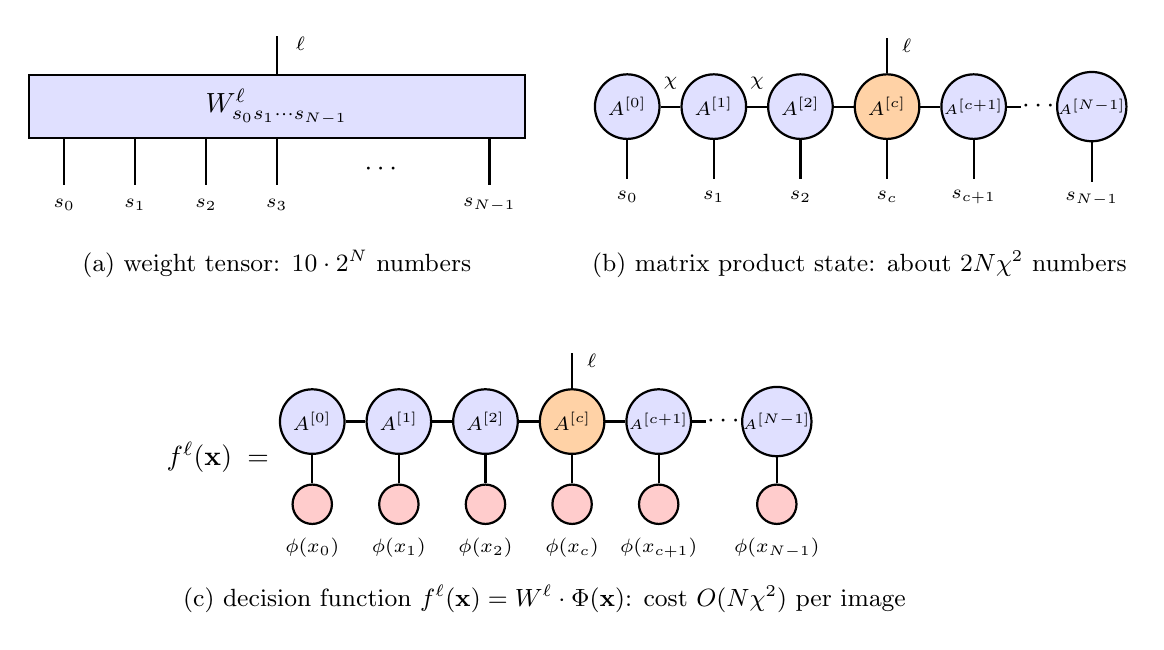
\begin{tikzpicture}
  % ---------------------------------------------------------------- (a) full weight tensor
  \begin{scope}[shift={(0,0)}]
    \draw[thick, fill=blue!12] (0,0) rectangle (6.3,0.8);
    \node at (3.15,0.4) {$W^{\ell}_{s_0 s_1\cdots s_{N-1}}$};
    \foreach \x/\s in {0.45/0,1.35/1,2.25/2,3.15/3} {\draw[thick] (\x,0) -- (\x,-0.6); \node[font=\scriptsize] at (\x,-0.85) {$s_{\s}$};}
    \node at (4.5,-0.4) {$\cdots$};
    \draw[thick] (5.85,0) -- (5.85,-0.6); \node[font=\scriptsize] at (5.85,-0.85) {$s_{N-1}$};
    \draw[thick] (3.15,0.8) -- (3.15,1.3); \node[font=\scriptsize] at (3.45,1.2) {$\ell$};
    \node[font=\small, align=center] at (3.15,-1.6) {(a) weight tensor: $10\cdot 2^N$ numbers};
  \end{scope}
  % ---------------------------------------------------------------- (b) MPS
  \begin{scope}[shift={(7.6,0.4)}]
    \foreach \i/\k/\x in {1/0/0,2/1/1.1,3/2/2.2} {\node[site] (a\i) at (\x,0) {$A^{[\k]}$};}
    \node[lab] (a4) at (3.3,0) {$A^{[c]}$};
    \node[site] (a5) at (4.4,0) {\tiny$A^{[c+1]}$};
    \node[site] (a6) at (5.9,0) {\tiny$A^{[N-1]}$};
    \draw[thick] (a1) -- (a2) -- (a3) -- (a4) -- (a5);
    \draw[thick] (a5) -- (5.0,0); \node at (5.25,0) {$\cdots$}; \draw[thick] (5.45,0) -- (a6);
    \node[font=\scriptsize] at (0.55,0.3) {$\chi$}; \node[font=\scriptsize] at (1.65,0.3) {$\chi$};
    \foreach \i in {1,...,6} {\draw[thick] (a\i.south) -- ++(0,-0.5);}
    \foreach \i/\s in {1/0,2/1,3/2,4/c,5/c+1,6/N-1} {\node[font=\scriptsize] at ($(a\i.south)+(0,-0.72)$) {$s_{\s}$};}
    \draw[thick] (a4.north) -- ++(0,0.45); \node[font=\scriptsize] at ($(a4.north)+(0.25,0.35)$) {$\ell$};
    \node[font=\small, align=center] at (2.95,-2.0) {(b) matrix product state: about $2N\chi^2$ numbers};
  \end{scope}
  % ---------------------------------------------------------------- (c) contraction with the data
  \begin{scope}[shift={(3.6,-3.6)}]
    \foreach \i/\k/\x in {1/0/0,2/1/1.1,3/2/2.2} {\node[site] (b\i) at (\x,0) {$A^{[\k]}$};}
    \node[lab] (b4) at (3.3,0) {$A^{[c]}$};
    \node[site] (b5) at (4.4,0) {\tiny$A^{[c+1]}$};
    \node[site] (b6) at (5.9,0) {\tiny$A^{[N-1]}$};
    \draw[thick] (b1) -- (b2) -- (b3) -- (b4) -- (b5);
    \draw[thick] (b5) -- (5.0,0); \node at (5.25,0) {$\cdots$}; \draw[thick] (5.45,0) -- (b6);
    \foreach \i/\s in {1/1,2/2,3/3,4/c,5/{},6/N} {\node[feat] (f\i) at ($(b\i)+(0,-1.05)$) {}; \draw[thick] (b\i.south) -- (f\i.north);}
    \foreach \i/\s in {1/0,2/1,3/2,4/c,5/c+1,6/N-1} {\node[font=\scriptsize] at ($(f\i)+(0,-0.55)$) {$\phi(x_{\s})$};}
    \draw[thick] (b4.north) -- ++(0,0.45); \node[font=\scriptsize] at ($(b4.north)+(0.25,0.35)$) {$\ell$};
    \node at (-1.2,-0.45) {$f^{\ell}(\mathbf{x})\;=$};
    \node[font=\small, align=center] at (2.95,-2.25) {(c) decision function $f^{\ell}(\mathbf{x})=W^{\ell}\cdot\Phi(\mathbf{x})$: cost $O(N\chi^2)$ per image};
  \end{scope}
\end{tikzpicture}
\end{document}
